\section*{Performanceanalyse}

\begin{center}
  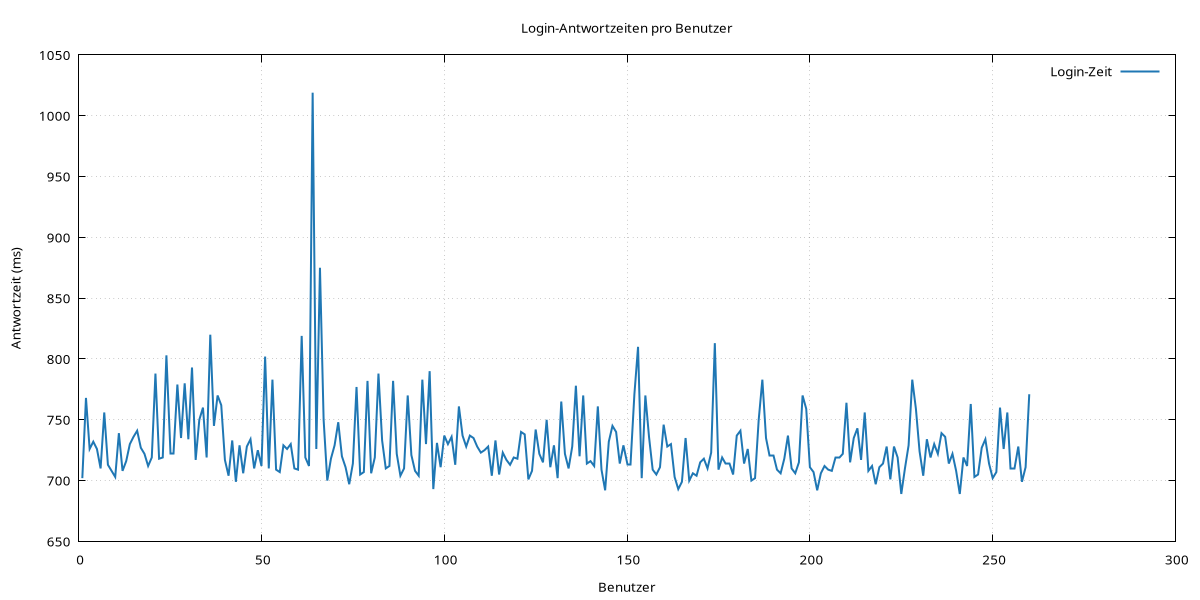
\includegraphics[width=0.95\linewidth, height=0.45\textheight, keepaspectratio]{src/abbildungen/login_lasttest.png}
  \captionof{figure}{Lasttest}
\end{center}

In unserem Lasttest wurden Login-Antwortzeiten mit steigender Benutzeranzahl gemessen. 
Für diesen Test wurden in Gruppen von 10, 25, 50, 75 und 100 Benutzern jeweils neue Testnutzer automatisch registriert und anschließend eingeloggt. Jeder Login wurde mit curl per HTTP-POST-Anfrage durchgeführt, wobei die Antwortzeit in Millisekunden 
sowie der HTTP-Statuscode erfasst wurde. Das Ziel war es, die Skalierbarkeit und Belastbarkeit des Systems im Bereich „Login“ zu analysieren, insbesondere unter der Annahme, dass bei hohem Nutzeraufkommen (wie in Pandemiesituationen) viele Benutzer innerhalb kurzer Zeit gleichzeitig auf das System zugreifen.
